%!TEX root = ../main.tex
\chapter{自旋与谐振腔耦合强度仿真}
\label{cha:spin_simulation}



        通过文献综述我们看到,单个自旋与常见谐振腔的耦合强度较弱,因此我们希望通过利用自旋系综与谐振腔进行耦合或者尝试新的谐振腔设计来解决这个问题。对自旋系综与谐振腔进行耦合的情况,由于自旋系综在空间有分布,而谐振腔所产生的磁场在空间也有所分布,因此探究谐振腔产生的磁场的空间分布即成为估计耦合系数的强度大小极其空间分布的重要步骤。

        另一方面,与平面波导谐振腔相对应,三维谐振腔的电磁场空间分布更均匀,但强度相对更弱,因此耦合强度更小。在尝试更新的谐振腔设计时,我们也考虑改良三维谐振腔使之在保持自旋系综存在空间部分电磁场仍旧相对均匀的同时尽可能增加场强,而对于平面波导谐振腔,我们从进一步增大耦合强度并与单个自旋耦合的角度出发在现有提案\cite{sarabi2017prospective}的基础上进行了仿真,改进与优化。

        \section{新型3D谐振腔与自旋系综的耦合} % (fold)
        \label{sec:新型3d谐振腔与自旋系综的耦合}

        我们首先发现并重复了对优化电磁场分布均匀性的3D谐振腔的仿真\cite{Angerer2016}。这种三维谐振腔中电流与磁场分布示意图如下图所示

        \begin{figure}[h]
                \centering
            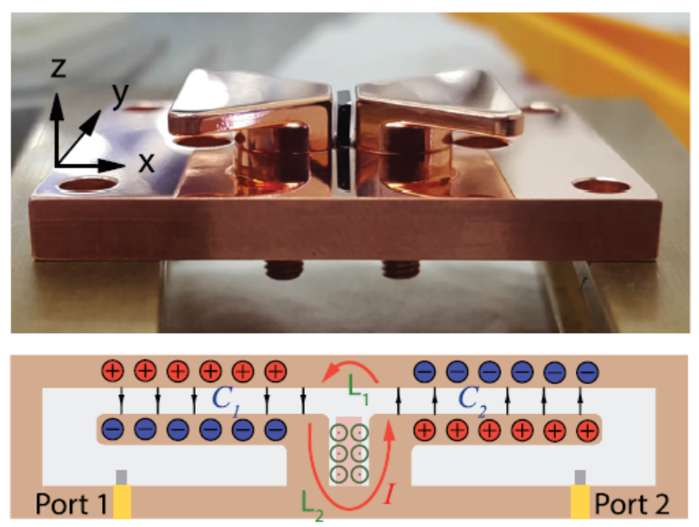
\includegraphics[width=4in]{3DResonator_image.png}
            \caption{新型三维谐振腔的几何结构与电流,磁场分布示意图\cite{Angerer2016}}
            \label{fig:3D_Resonator_image}
        \end{figure}
        其中这种三维谐振腔在普通密闭金属盒构成的三维谐振腔的基础上将电场与磁场局限于更小的体积当中,电场主要分布于两个扇形与盒顶之间,磁场主要分布于两扇形竖直支撑部分的两个平面之间,也为固定自旋系综的空间区域。因此这种三维谐振腔通过减小模式体积提高了零场涨落的大小,并同时仍保证自旋系综与磁场有较为均匀的耦合。


        \begin{figure}[h]
                \centering
            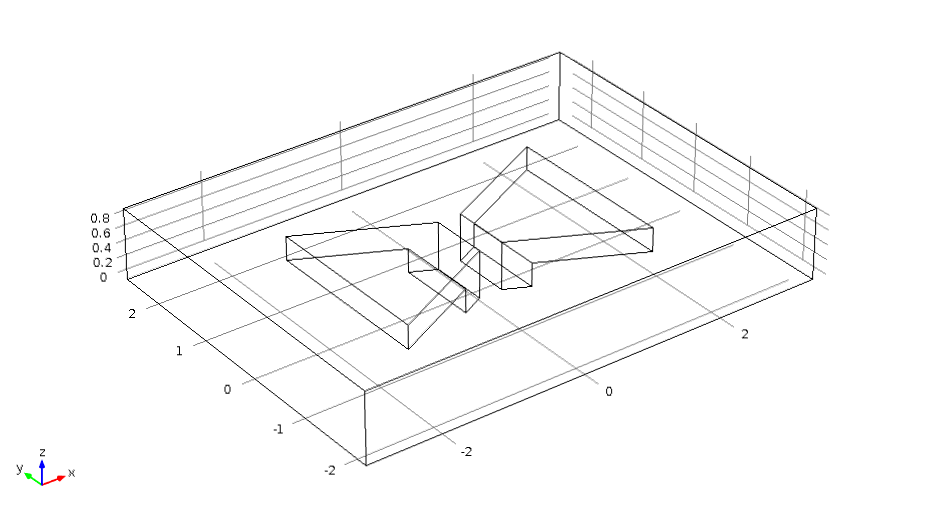
\includegraphics[width=4in]{geo.png}
            \caption{新型三维谐振腔仿真的几何设计(透视图)}
            \label{fig:geo_3DResonator}
        \end{figure}

        \begin{figure}[h]
                \centering
            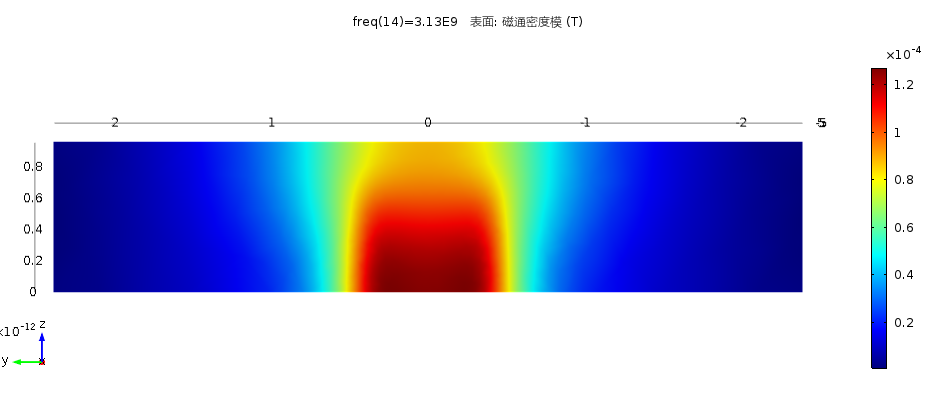
\includegraphics[width=4.5in]{normB_cross_sec_mid_yz_3.13GHz_smooth.png}
            \caption{新型三维谐振腔磁场在自旋系综所处空间横截面上的大小分布}
            \label{fig:sim_result_BField_crossSection}
        \end{figure}

        通过对Angerer等人使用的三维谐振腔的观察,我设计了如图\ref{fig:geo_3DResonator}所示几何形状的三维谐振腔。利用COMSOL求解谐振腔中电磁场的分布,能够得到自旋系综所在的横截面上的磁场分布如图\ref{fig:sim_result_BField_crossSection}所示。谐振腔的频率响应为频率和衰减率的函数\cite{grezes2016towards}
        \begin{equation}
            |S_{21}|^2 = \left | \frac{i \kappa/2}{2 \pi (\delta f - \delta f_c)+i (\kappa + \kappa_L)/2 } \right|^2
        \end{equation}
        通过对仿真所得的谐振腔的频率响应进行拟合,能够得到谐振腔的衰减率$ \kappa, \kappa_L $,进而求出对应任意功率下的谐振腔中的光子数\cite{grezes2016towards}
        \begin{equation}
            n = \frac{2 \kappa}{h f_c (\kappa+ \kappa_L)^2} P
        \end{equation}
        谐振腔中仿真的场与功率相关,知道给定功率下的谐振腔中的电磁场分布,以及相应腔内光子数后,即可简单计算得单位光子数对应的电磁场大小与分布。通过单位光子数的磁场大小,即可计算自旋与谐振腔中该模式的耦合强度\cite{Angerer2016}
        \begin{equation}
            |g_0| = \sqrt{\frac{2}{3}} \frac{\mu_B g_e}{2\hbar} |\bm B_0||\bm S| \sim 100 \mathrm{mHz}
        \end{equation}

        通过仿真,拟合与计算得到的耦合强度,与Angerer等人所得到的耦合强度的数量级相符,验证了我们的仿真与计算的正确性。综合考虑后,我们认为这种方法对耦合强度的增加不明显,没有数量级的提升,并且这种三维谐振腔的制备较为复杂,我们没有继续进行这种新型三维谐振腔的制备。
        
        
        





        \section{2D平面波导谐振腔与自旋系综的耦合} % (fold)
        \label{sec:2d平面波导谐振腔与自旋系综的耦合}

        目前有很多工作通过将自旋系综与二维平面波导谐振腔进行耦合,达到了强耦合的效果\cite{kubo2010,Schuster2010}。对于这类耦合,谐振腔的耦合强度的大小及其分布依赖于电磁场的空间分布。因此,我对二维平面波导的电磁场的空间分布进行了仿真,并与文献进行了比较。

        对于二维平面波导的仿真,空间中场的分布由金属中电流密度的分布决定,因此仿真的关键为得到可靠的电流密度分布,从而得到空间中场的分布。超导效应对金属中场的分布体现在电流穿透金属表面的深度有限,即与高频电流导致的趋肤效应十分类似,因此可通过高频电流的趋肤效应对超导电流的分布进行模拟\cite{Mark2013}。趋肤效应的深度电流频率相关:
        \begin{equation}
            \lambda_{skin} = \sqrt{\frac{2}{\sigma \omega \mu}}
        \end{equation}
        通过使趋肤效应的深度等于超导电流的穿透深度,我们估计得仿真所需采用的电流频率为$ \omega \approx 660 $GHz。这个频率并不对应实际物理系统中的任何频率,仅为仿真所采用的一个参数。零场涨落下的电磁场分布直接通过使总电流的大小为零场电流涨落的大小来得到。零场电流的大小通过计算可得\cite{PhysRevA.95.022306,Mark2013,Tosi2014}
        \begin{align}
            \label{eqn:ZPF_estimation}
            \frac{\hbar \omega }{2} &= 2\times \frac{1}{2}L (\delta i_{rms})^2\\
            L&= \frac{2Z_0}{\pi \omega}\\
            \delta i_{rms } &= \omega \sqrt{ \frac{\hbar \pi}{4Z_0} }\approx 50 \mathrm{nA}
        \end{align}
        
        通过上述方法,我采用了与两篇文章中相同的器件几何尺寸对磁场进行了仿真,如图所示。


        \begin{figure}
            \begin{minipage}[b]{0.4\textwidth}
                \centering
                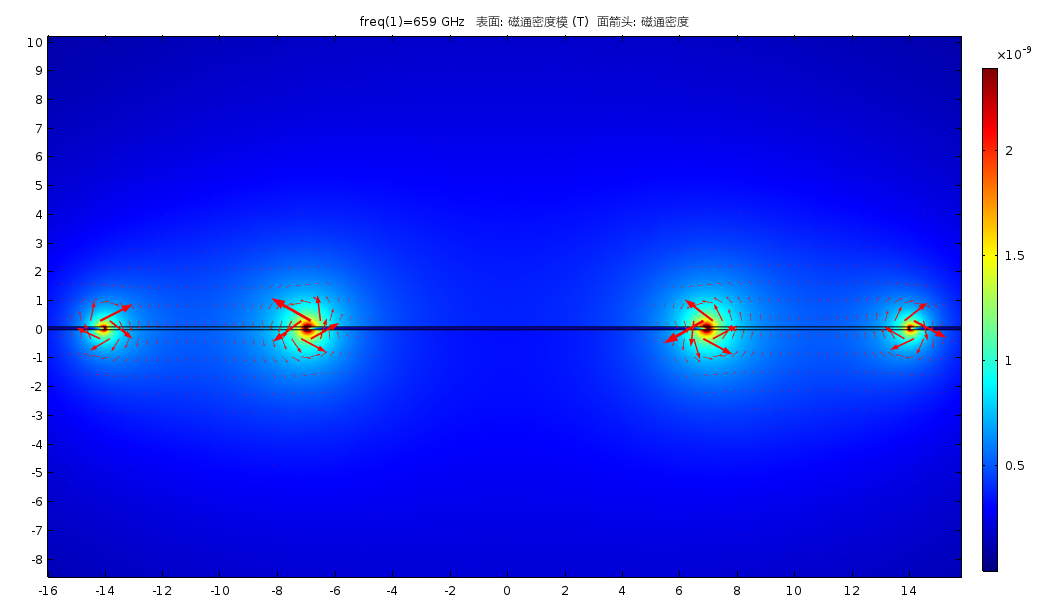
\includegraphics[width=3in]{20161122_Bnorm_cross_659GHz.png}
                \caption{仿真所得磁场空间分布截面图}
                \label{fig:20161122_Bnorm_cross_659GHz}
            \end{minipage}%
            % \hspace{0.1\textwidth}%
            % \hfill
            \hspace*{\fill}
            \begin{minipage}[b]{0.5\textwidth}
                \centering
                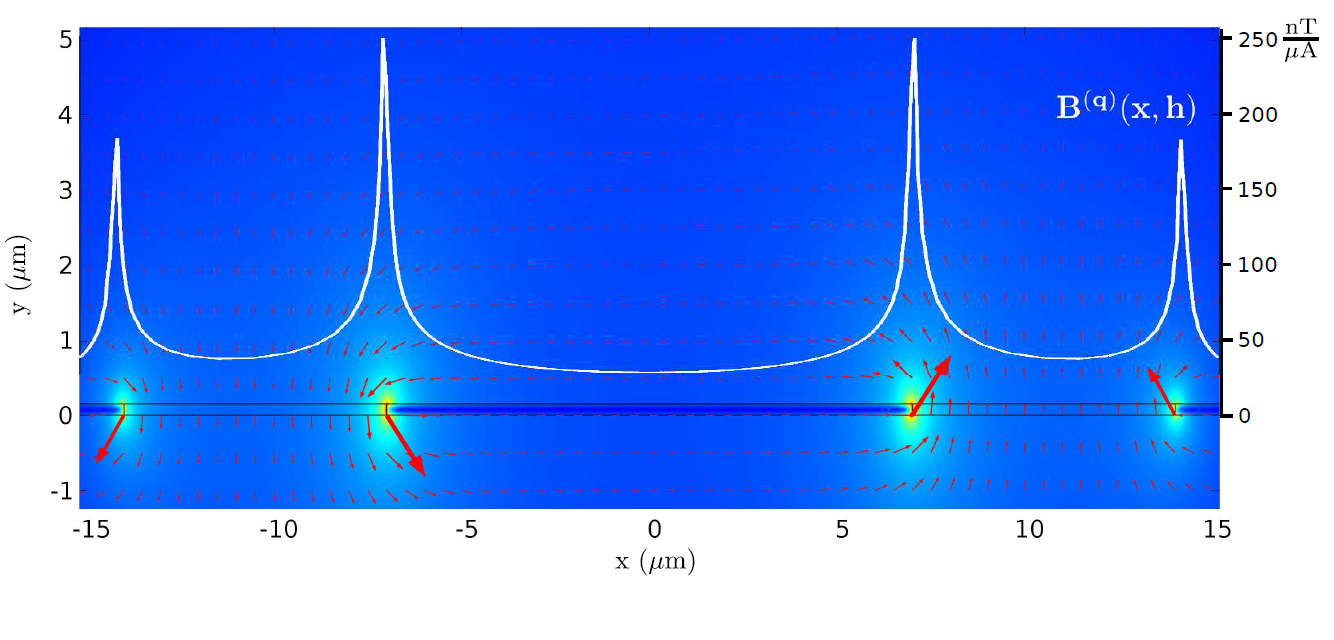
\includegraphics[width=3.5in]{Coupling-SMM-to-quantum-circuits-fig7.png}
                \caption{文献\cite{Mark2013}中所示磁场空间分布截面图}
                \label{fig:Coupling-SMM-to-quantum-circuits-fig7}
            \end{minipage}
        \end{figure}
        
        \begin{figure}
            \begin{minipage}[b]{0.4\textwidth}
                \centering
                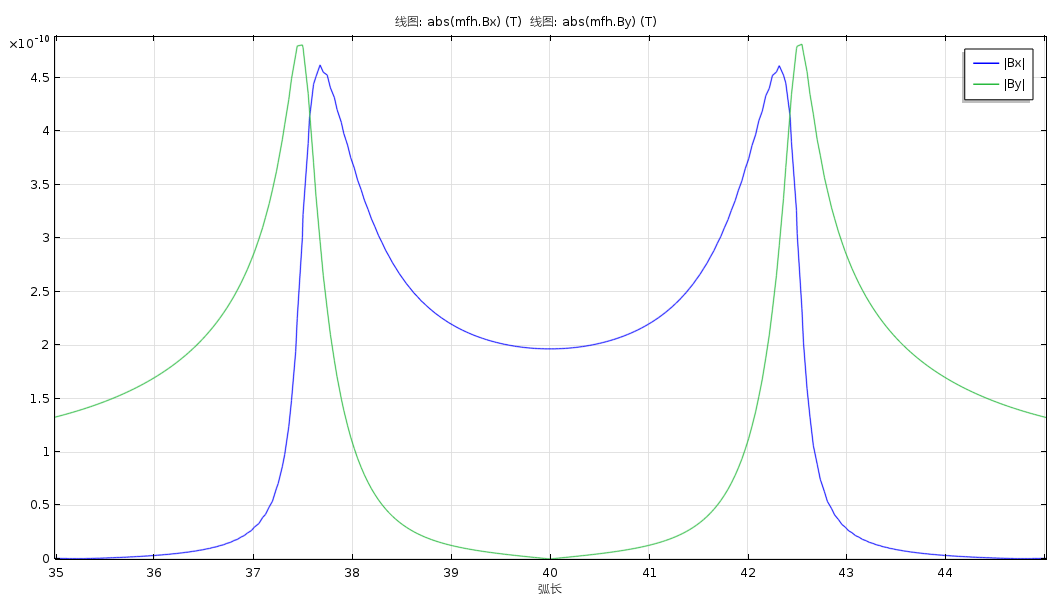
\includegraphics[width=3in]{20161122-2_Bxy_0.1um_below_659GHz.png}
                \caption{仿真所得磁场在位于距金属上表面$0.1\mu m$处水平截线上的分布}
                \label{fig:20161122-2_Bxy_0.1um_below_659GHz}
            \end{minipage}%
            % \hspace{0.1\textwidth}%
            % \hfill
            \hspace*{\fill}
            \begin{minipage}[b]{0.5\textwidth}
                \centering
                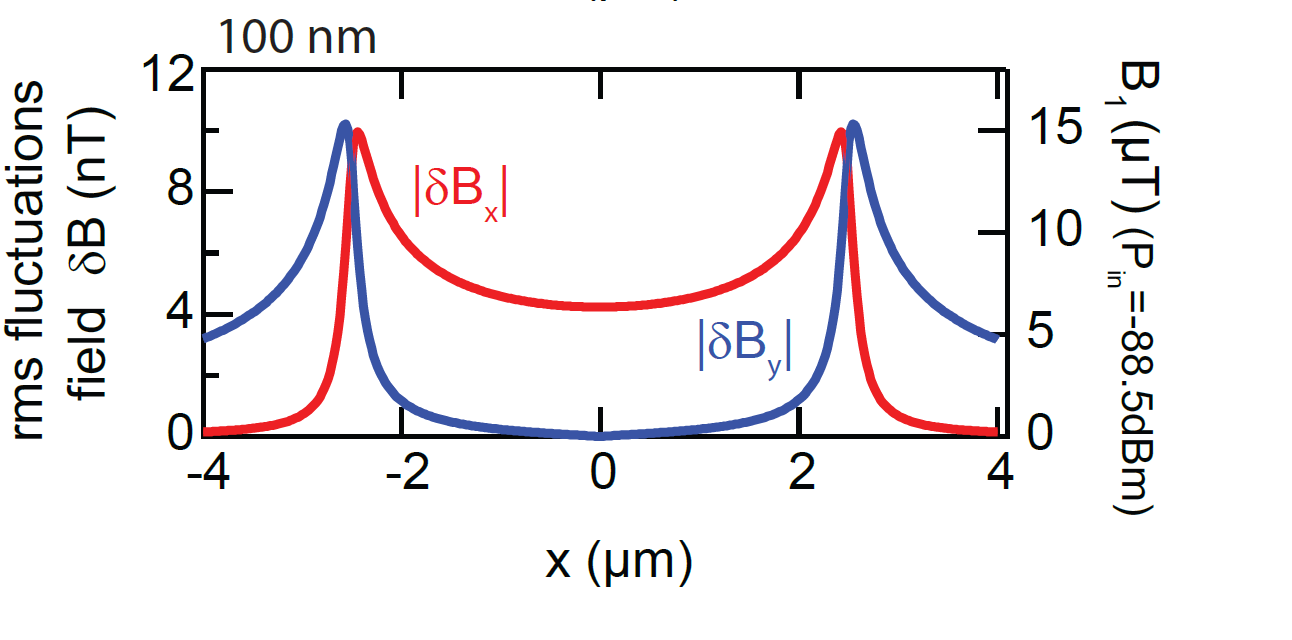
\includegraphics[width=3.5in]{Reaching-the-quantum-limit-of-sensitivity-SI-fig3d.png}
                \caption{文献\cite{Bienfait2016a}中所示磁场在位于距金属上表面$0.1\mu m$处水平截线上的分布}
                \label{fig:Reaching-the-quantum-limit-of-sensitivity-SI-fig3d}
            \end{minipage}
        \end{figure}
        

        通过利用上述方法对两篇独立的文章中的几何结构进行仿真并且与文章中的结果比较,可以看出结果相符。验证上述方法的可行性后,我对我们制备的二维平面波导的常见几何尺寸进行了仿真,并绘制了距离波导金属表面不同高度处的水平截线上的磁感应强度分布,如图\ref{fig:20161122-2_Bnorm_lines_659GHz}所示。

        \begin{figure}[h]
                \centering
            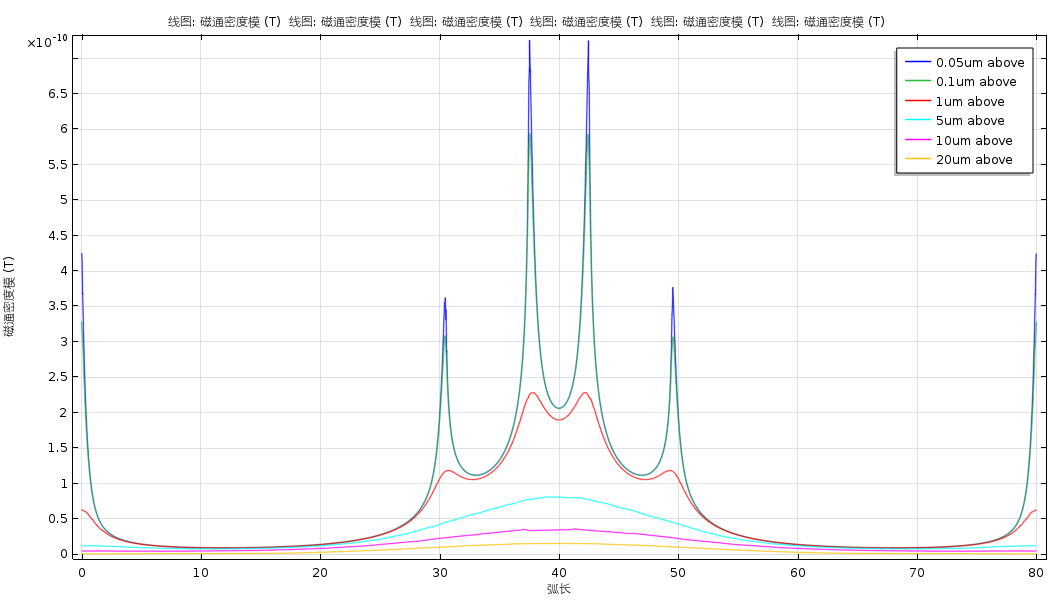
\includegraphics[width=4.5in]{20161122-2_Bnorm_lines_659GHz.png}
            \caption{基于我们制备的二维平面波导的常见几何尺寸进行仿真所得的磁感应强度分布图。}
            \label{fig:20161122-2_Bnorm_lines_659GHz}
        \end{figure}

        通过仿真结果可以看出,磁场在金属上方$10 \mathrm{\mu m}$左右的范围内开始分布均匀,并且强度在$ 0.5\times 10^{-10} $T的范围左右,对应的耦合强度$ g \sim 2 \pi \cdot 10 $Hz,与文献中对单个自旋与二维平面波导谐振腔的耦合常数的估计值相符很好。因此,通过这种仿真方法,我们能够很快得到给定任意几何形状的二维平面波导的空间磁场分布,进而得到空间内任意一点处的自旋与基于该二维平面波导构成的谐振腔的模式的耦合强度。







        \section{螺旋状电感谐振腔与2.5维谐振腔与单个自旋的耦合} % (fold)
        \label{sec:螺旋状电感与2_5d谐振腔与单个自旋的耦合}

            前面讨论了利用与自旋系综耦合来增大耦合常数。通过观察耦合常数的表达式\ref{eqn:coupling_coeff},可以看见还可以通过提高零场涨落的大小来提高单个自旋与谐振腔模式的耦合常数。


            \subsection{参数估计} % (fold)
            \label{sub:参数估计}

                通过对零场电流大小进行估计的\ref{eqn:ZPF_estimation}式,可以看到零场电流涨落
                \begin{equation}
                    \delta I = \sqrt{ \frac{\hbar \omega}{2 L} }
                \end{equation}
                而对于选定的自旋种类以及基于选定自旋的能级系统定义出的二能级量子比特,其能级间能量差大致固定,因此谐振腔的谐振频率也大致固定在该能量所对应的频率。而谐振腔的频率由$ \omega = 1/\sqrt{LC} $确定。通过上述讨论可以看到,通过增大零场电流涨落可以增大磁场,进而增大单个自旋与谐振腔模式的耦合常数,增大零场电流涨落可由减小谐振腔的电感$L$实现,而对于固定频率的谐振腔,减小$L$意味着增大电容$C$。如果我们想要达到的耦合强度$ g/2 \pi \sim 1 \mathrm{MHz} $,并且利用如基于金刚石色心的能量差对应频率在$3 \mathrm{GHz} $左右的自旋系统,可以估计出相应的零场电流涨落,对应的谐振腔电感与电容的数量级为
                \begin{align}
                    \delta I & \sim  1 \mathrm{\mu A}\\
                    L & \sim  1 \mathrm{pH}\\
                    C & \sim  1 \mathrm{nF}
                \end{align}
                对于nF数量级的电容,无法通过如齿状二维电容等二维设计实现,而可使用三维平板电容实现。因此,我把这种电感为二维结构而电容为三维结构的谐振腔称为2.5维谐振腔。已有研究人员提出基于这种思路设计的2.5维谐振腔\cite{sarabi2017prospective},我基于他们的谐振腔设计进行了仿真与优化。
                

                
            \subsection{电感设计与优化} % (fold)
            \label{sub:电感设计与优化}

                对于2.5维谐振腔的电感部分,Sarabi等人提出的设计如图\ref{fig:spiral_proposal_1}所示。


            \begin{figure}
                \begin{minipage}[b]{0.4\textwidth}
                    \centering
                    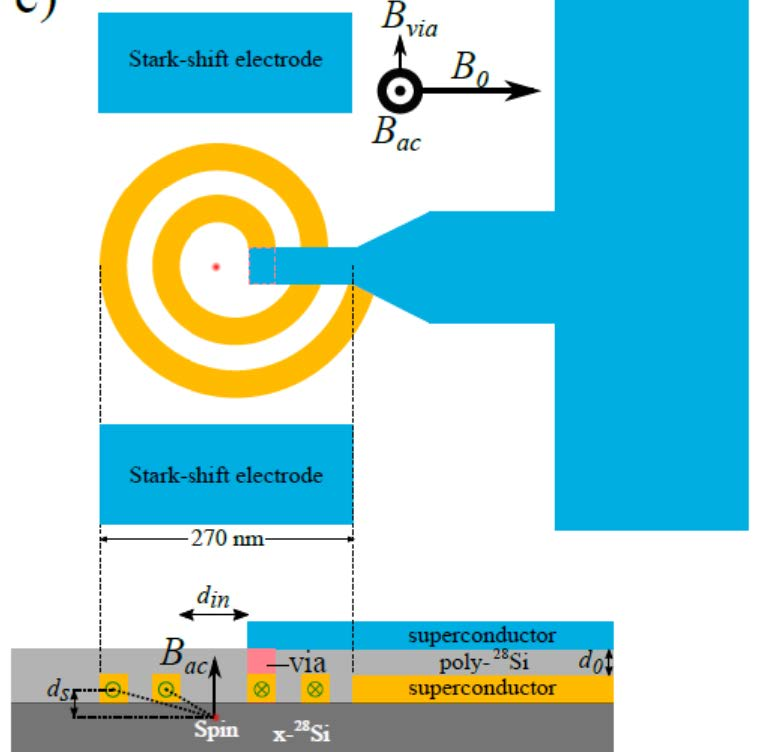
\includegraphics[width=3in]{spiral_proposal_1.jpg}
                    \caption{来自参考文献~\inlinecite{sarabi2017prospective}的2.5维谐振腔的设计(右图中红色虚线部分的局部放大图)。}
                    \label{fig:spiral_proposal_1}
                \end{minipage}%
                % \hspace{0.1\textwidth}%
                % \hfill
                \hspace*{\fill}
                \begin{minipage}[b]{0.5\textwidth}
                    \centering
                    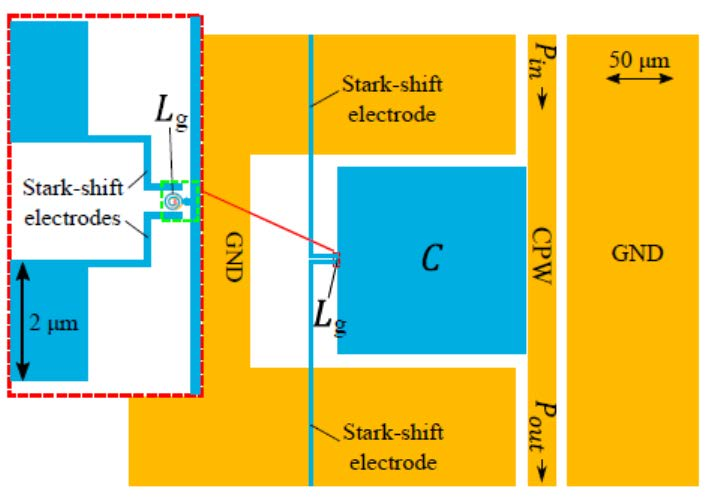
\includegraphics[width=3.5in]{spiral_proposal_2.jpg}
                    \caption{来自参考文献~\inlinecite{sarabi2017prospective}的2.5维谐振腔的设计(整体)。}
                    \label{fig:spiral_proposal_2}
                \end{minipage}
            \end{figure}
            其中主要图示均为俯视图,左图的下方的小图为横截面示意图。右图中蓝色的部分即为层状电容的俯视图。通过根据相关几何参数进行仿真,我得到了这种谐振腔的电感部分的磁场分布图,如图\ref{fig:res_spiral_normB_xy_20170314}所示。通过分析我们发现,耦合系数能够得到数量级上的提升的根本原因是选取了很小的电感$L$,从而得到了较大的零场磁场涨落,并且自旋距离电感部分导线的距离较近,为$~10$nm的数量级。而与之相对的,螺旋状电感的螺旋圈数则相对不那么重要,不会对耦合强度产生数量级上的影响,反而加大了微纳加工制备的难度。因此,我们进一步对螺旋状电感进行了分析,改良与仿真。

            \begin{figure}[h]
                \centering
                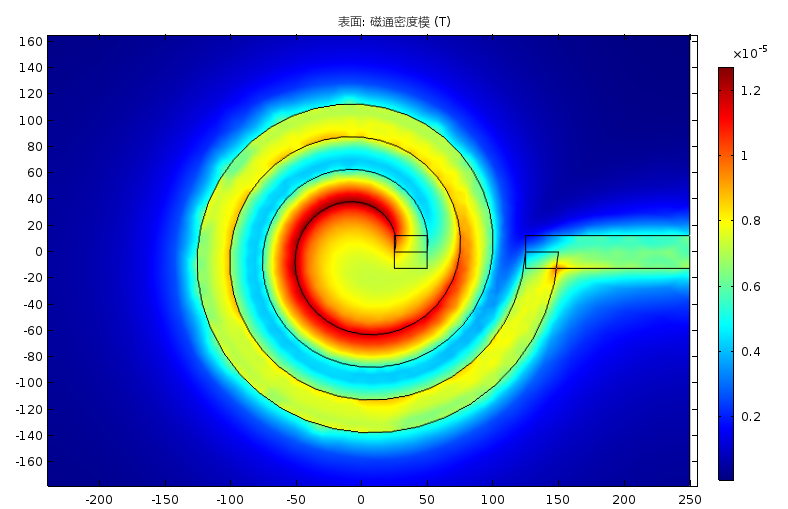
\includegraphics[width=4in]{res_spiral_normB_xy_20170314.png}
                \caption{2.5维谐振腔的螺旋状电感处水平截面上的磁感应强度分布。}
                \label{fig:res_spiral_normB_xy_20170314}
            \end{figure}

            \begin{figure}[h]
                \centering
                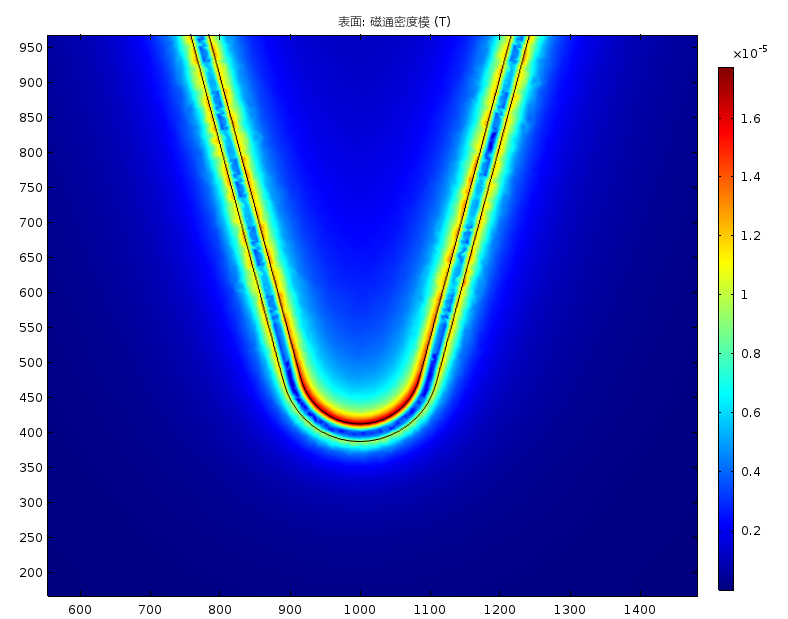
\includegraphics[width=3in]{res_UInd_normB_20170317.png}
                \caption{第一次改进后的2.5维谐振腔的电感处水平截面上的磁感应强度分布。}
                \label{fig:res_UInd_normB_20170317}
            \end{figure}


            \begin{figure}[h]
                \centering
                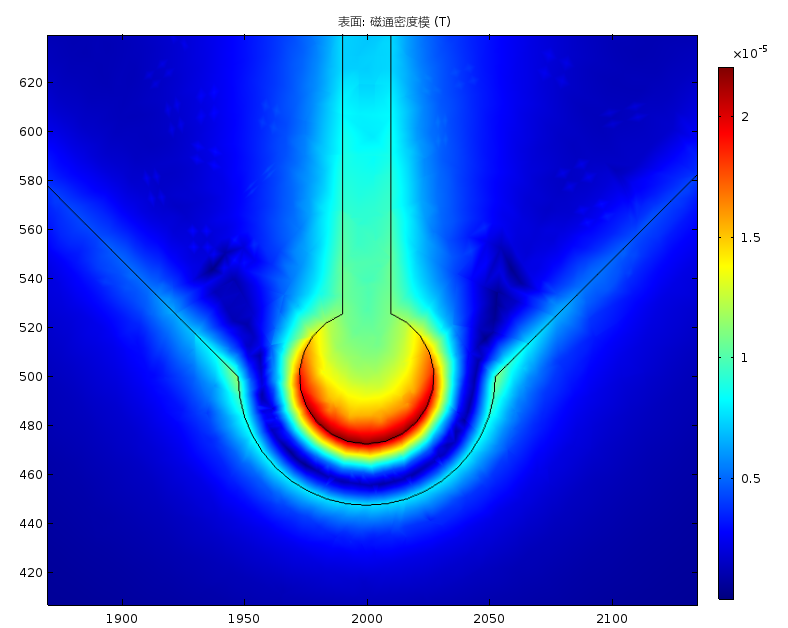
\includegraphics[width=3in]{res_UIndV3_normB_20170321.png}
                \caption{第二次改进后的2.5维谐振腔的电感处水平截面上的磁感应强度分布,电感部分的电感大小得到了降低。}
                \label{fig:res_UIndV3_normB_20170321}
            \end{figure}

            

            \begin{figure}[h]
                \centering
                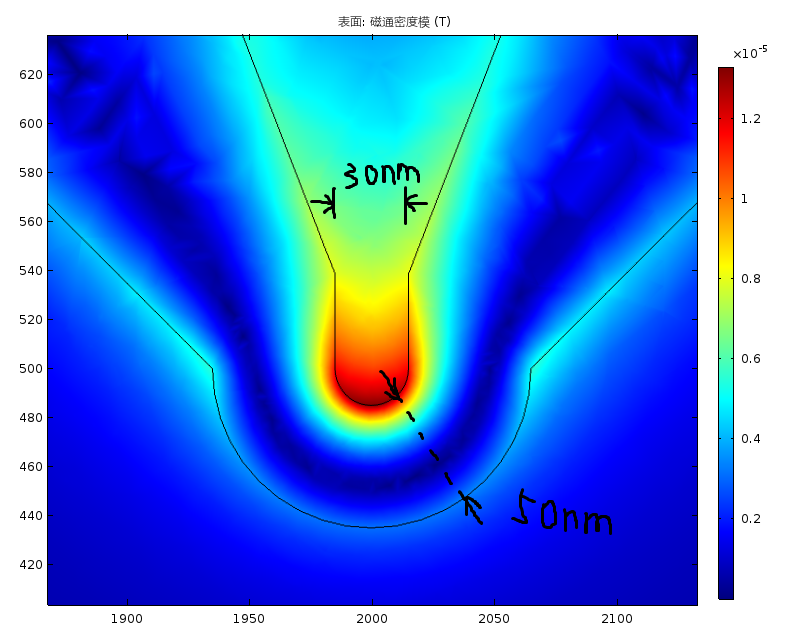
\includegraphics[width=3in]{res_UIndV4_50nm_normB_20170406.png}
                \caption{第三次改进后的2.5维谐振腔的电感处水平截面上的磁感应强度分布,通过加厚材料并加粗宽度提升了临界电流大小,并在不影响磁场较强区域的强度的基础上改进了设计以提高制备的成功率。}
                \label{fig:res_UIndV4_50nm_normB_20170406}
            \end{figure}


            首先,我简化了螺旋状的电感结构,直接采用一根细导线作为电感,并通过磁场仿真来估算电感的数量级,仿真结果如图\ref{fig:res_UInd_normB_20170317}所示。通过仿真估算得到的电感值为$L\approx 2\times 10^{-12} \mathrm{H} $,比理想的电感值多出一倍左右。考虑到所需的强磁场区域并不需要分布于整个电感导线,而只需要在圆弧附近即可,而强磁场存在的区域更大自然会增大导线的自感。基于这个想法,我进一步改进了电感的几何设计,仅保留电感中间的圆弧部位较细,这样电流密度增大,磁场相应增大,而对于电流流入与流出圆弧部位的部分,使导线变宽,如图\ref{fig:res_UIndV3_normB_20170321}所示,即可减小大部分区域的磁场大小。通过仿真得出,电感大小的确减小到$L \approx 7\times 10^{-13} \mathrm{H} $,减小超过50\%。

            通过进一步讨论并考虑到测量系统的温度下限对应的噪声大小,我们希望谐振腔中能有远多于100个光子的信号。通过简单估计我们发现对于图\ref{fig:res_UIndV3_normB_20170321}以及其之前的结构,达到理想的光子数会使电流密度超过所用材料的超导临界电流密度,这样极有可能使器件损耗大大增加,并且因非超导态的电阻发热使电感部分的细导线烧断,导致器件损毁,因此需要进一步改进设计使同样临界电流密度的材料能够承载更多的电流。另一方面,图\ref{fig:res_UIndV3_normB_20170321}的设计由于电感环状结构的前后为尽可能增大导线宽度使输入与输出导线中部距离十分靠近,为$\sim 10 \mathrm{nm} $的数量级,在微纳加工过程中极易连接起来,在实际测试中也出现输入与输出两部分连接起来的现象。考虑上述两个因素后,我进一步改进了电感的设计,通过加厚材料并加宽导线圆弧部分,提高了可承载总电流的大小,并使导线的输入与输出部分分离更远距离,提高了制备的成功率。最终的电感设计如图\ref{fig:res_UIndV4_50nm_normB_20170406}所示。

            
            对于COMSOL仿真所得电感的准确度,我通过变化求解空间区域大小与网格致密程度,以及与经验公式相比较这两种方法进行了探究。对于矩形截面的直导线,其自感的计算公式为\cite{grover2004inductance}

            \begin{equation}
                \label{eqn:SelfInductance}
                L = 0.002l \left [ \ln \frac{2l}{B+C} + \frac{1}{2} - \ln(e) \right ]
            \end{equation}
            其中$B$,$C$为导线矩形横截面的边长,$l$为导线的长度,以厘米为单位,这样计算出的电感的单位为$ \mu  $H。最后一项$\ln(e)$并不等于一,需查表得知,但其值基本为$0.001$,对于当前的估计的精度而言可以忽略。
            

            通过仿真几何结构为20nm~x~20nm~x~250nm的直导线的自感,不同求解区域大小下COMSOL计算所得的电感值以及经验公式估计所得的电感值如表\ref{tab:InductanceComparison}所示。


\begin{table}[htb]
  \centering
  \caption{不同大小求解区域下COMSOL仿真所得电感值与经验公式估计的电感值}
  \label{tab:InductanceComparison}
    \begin{tabular}{c|cccc} %{\linewidth}{lX}
      \toprule %[1.5pt]
      求解区域 & $250^2\times 250$nm$^3$ & $500^2\times 250$nm$^3$ & $1000^2\times 250$nm$^3$ & 经验公式 \\
      \midrule %[1pt]
      电感值(H) & $1.378\times 10^{-13} $ & $1.705\times 10^{-13} $ & $2.019\times 10^{-13} $ & $1.512\times 10^{-13} $  \\
      \bottomrule %[1.5pt]
    \end{tabular}
\end{table}

        
        从表\ref{tab:InductanceComparison}中可以看出,COMSOL仿真的电感值随求解区域有较明显变化,但能够得到与经验公式数量级相符的结果。实际使用的电感也较为复杂,通过COMSOL的仿真与经验公式的估算也仅能给出一个参考值,具体还需通过实际制备出的器件积累数据与经验。

    